\frame{
	\insertsection{Introduction}
}

\begin{frame}
	\frametitle{Throwback}
	\framesubtitle{Pipeline spills, greenwashing, organizational learning}
	\begin{figure}
		\centerline{
			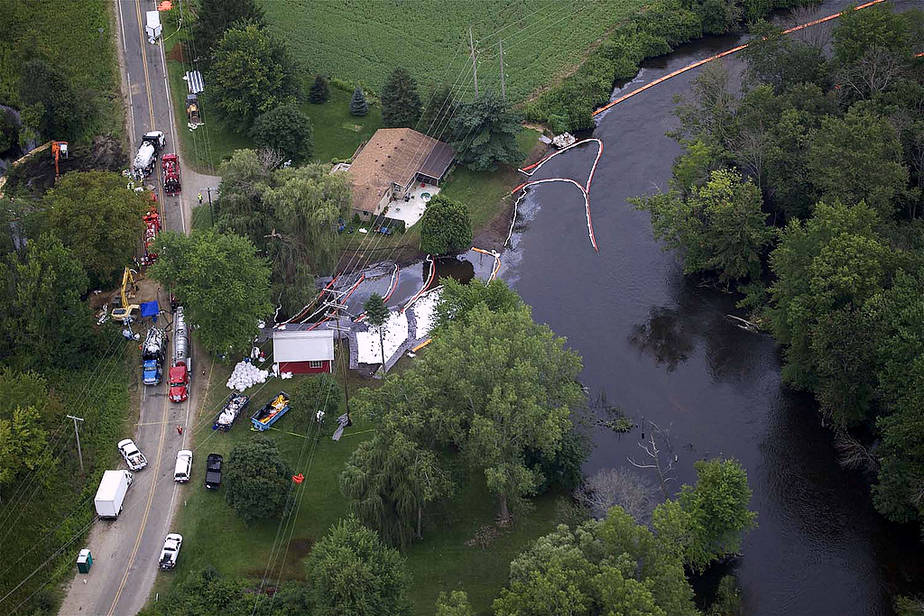
\includegraphics[scale=0.28]{kalamazoo.jpg}}
		\caption{\url{https://insideclimatenews.org/news/03052018/enbridge-fined-tar-sands-oil-pipeline-inspections-kalamazoo-michigan-dilbit-spill}}
	\end{figure}
	\note{
		The most real example of environmental pollution that I can think of. Quite countable. That is not to say that there isn't complexity, but it is very tangible. I think nobody calls pipeline spills fake news. Environmental pollution is my motivation.
	}
\end{frame}

\begin{frame}
	\frametitle{Tension}
	Technology \& Social-Ecological Systems
	\begin{figure}
		\centerline{
			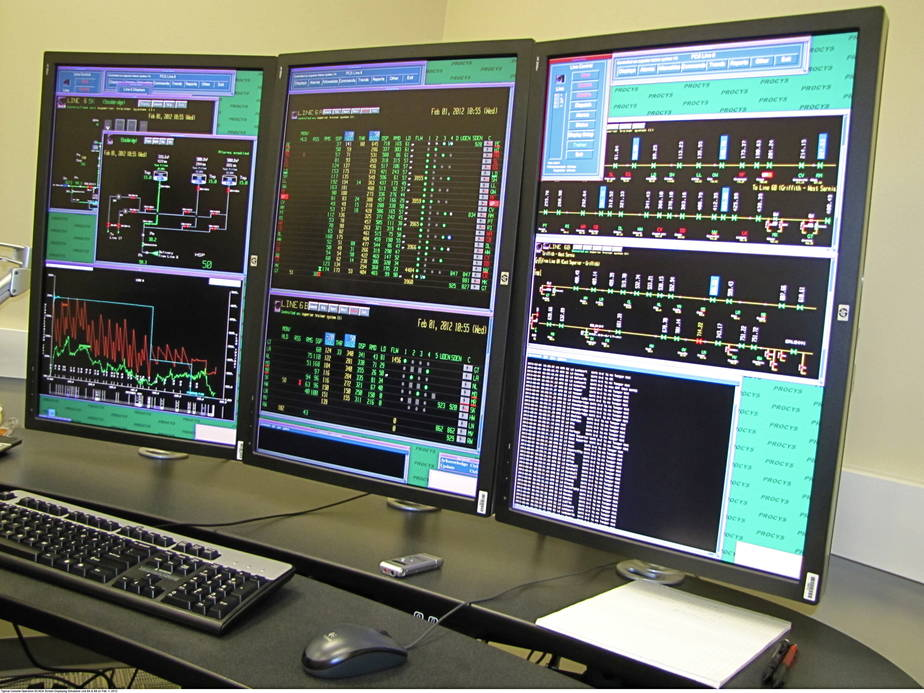
\includegraphics[scale=0.25]{scada.jpg}}
		\caption{\url{https://insideclimatenews.org/news/20120919/few-oil-pipeline-spills-detected-much-touted-technology}}
	\end{figure}
	\note{
		Great technology in pipelines. Not too complex, which is not to say ineffective. I can understand. You can understand. But at the same time, pipeline spills are still common place. How is that?
	}
\end{frame}

\begin{frame}
	\frametitle{Framework}
	Juxtapose communication and reality of pipeline safety:
	
	\begin{enumerate}
		\item <1-> Reliability: The pipeline industry communicates a complex shared understanding of pipeline safety.
		\item <2> Validity: Over the last 20 years, developments in pipeline safety does not address sources of pipeline spill.
	\end{enumerate}
	\vspace{0.1cm}
	\hrule
	\vspace{0.1cm}
	\citeauthor{Rerup2020} (forthcoming)
	\note{
		Juxtaposing two concepts that are a pair. Allows for talking about politics of pipeline safety through vehicle of greenwashing--reliability. And for looking into causes of pipeline spills, incident reports--validity.
		
		So mentally that is my structure, the idea that guides me through my dissertation. How far I will make that explicit though, I do not know yet.
	}
\end{frame}

\begin{frame}
	\frametitle{Phenomenon}
	\framesubtitle{Challenge 1: Communicate development in spill metrics}
	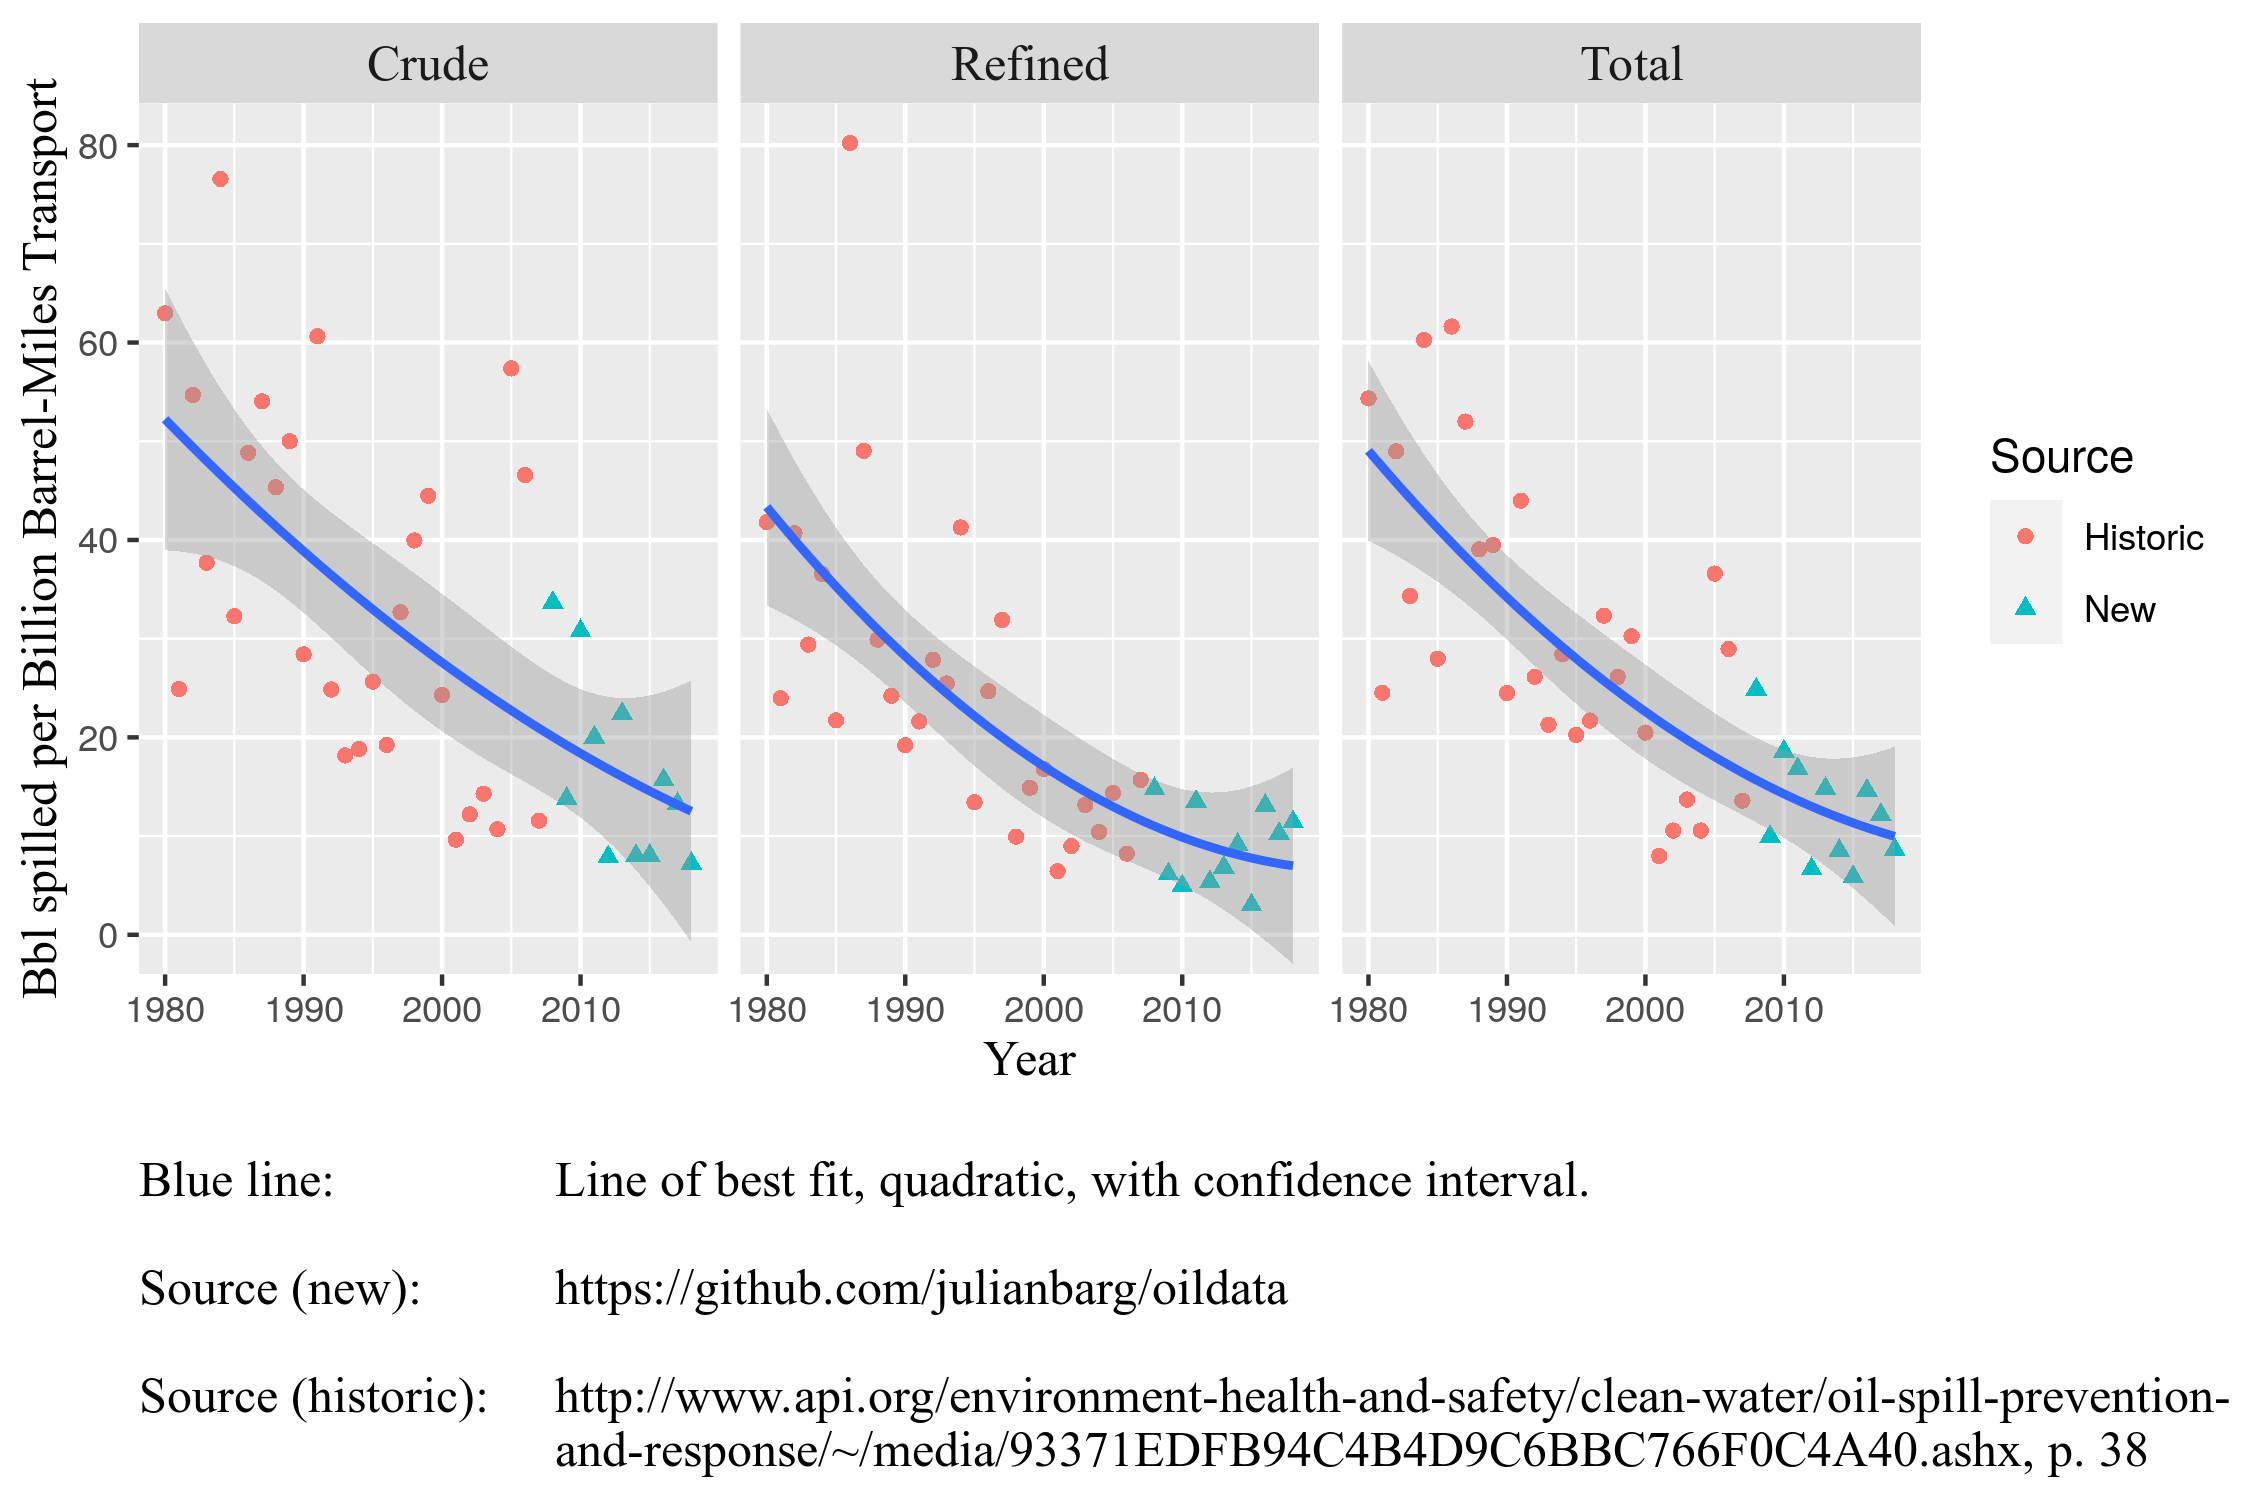
\includegraphics[scale=0.45]{population_learning_4.png}
	
	\note{
		We can see three things clearly. 
		
		\begin{enumerate}
			\item Crude pipelines show almost continuously improvements.
			\item Refined shows improvements into the early 2000s, then stays constant.
			\item For refined, it is hard to say whether there is one curve going on, or whether there is a decline, and then a standstill.
		\end{enumerate}
	
		Meaning that the reason for improvements in pipeline safety after 2000 is something that is specific to crude oil. Also, refined learning curve for post-2000 is indistinguishable from standstill. What has changed since the year 2000?
	}
\end{frame}

\begin{frame}
	\frametitle{Phenomenon}
	\framesubtitle{Challenge 1: Communicate development in spill metrics}
	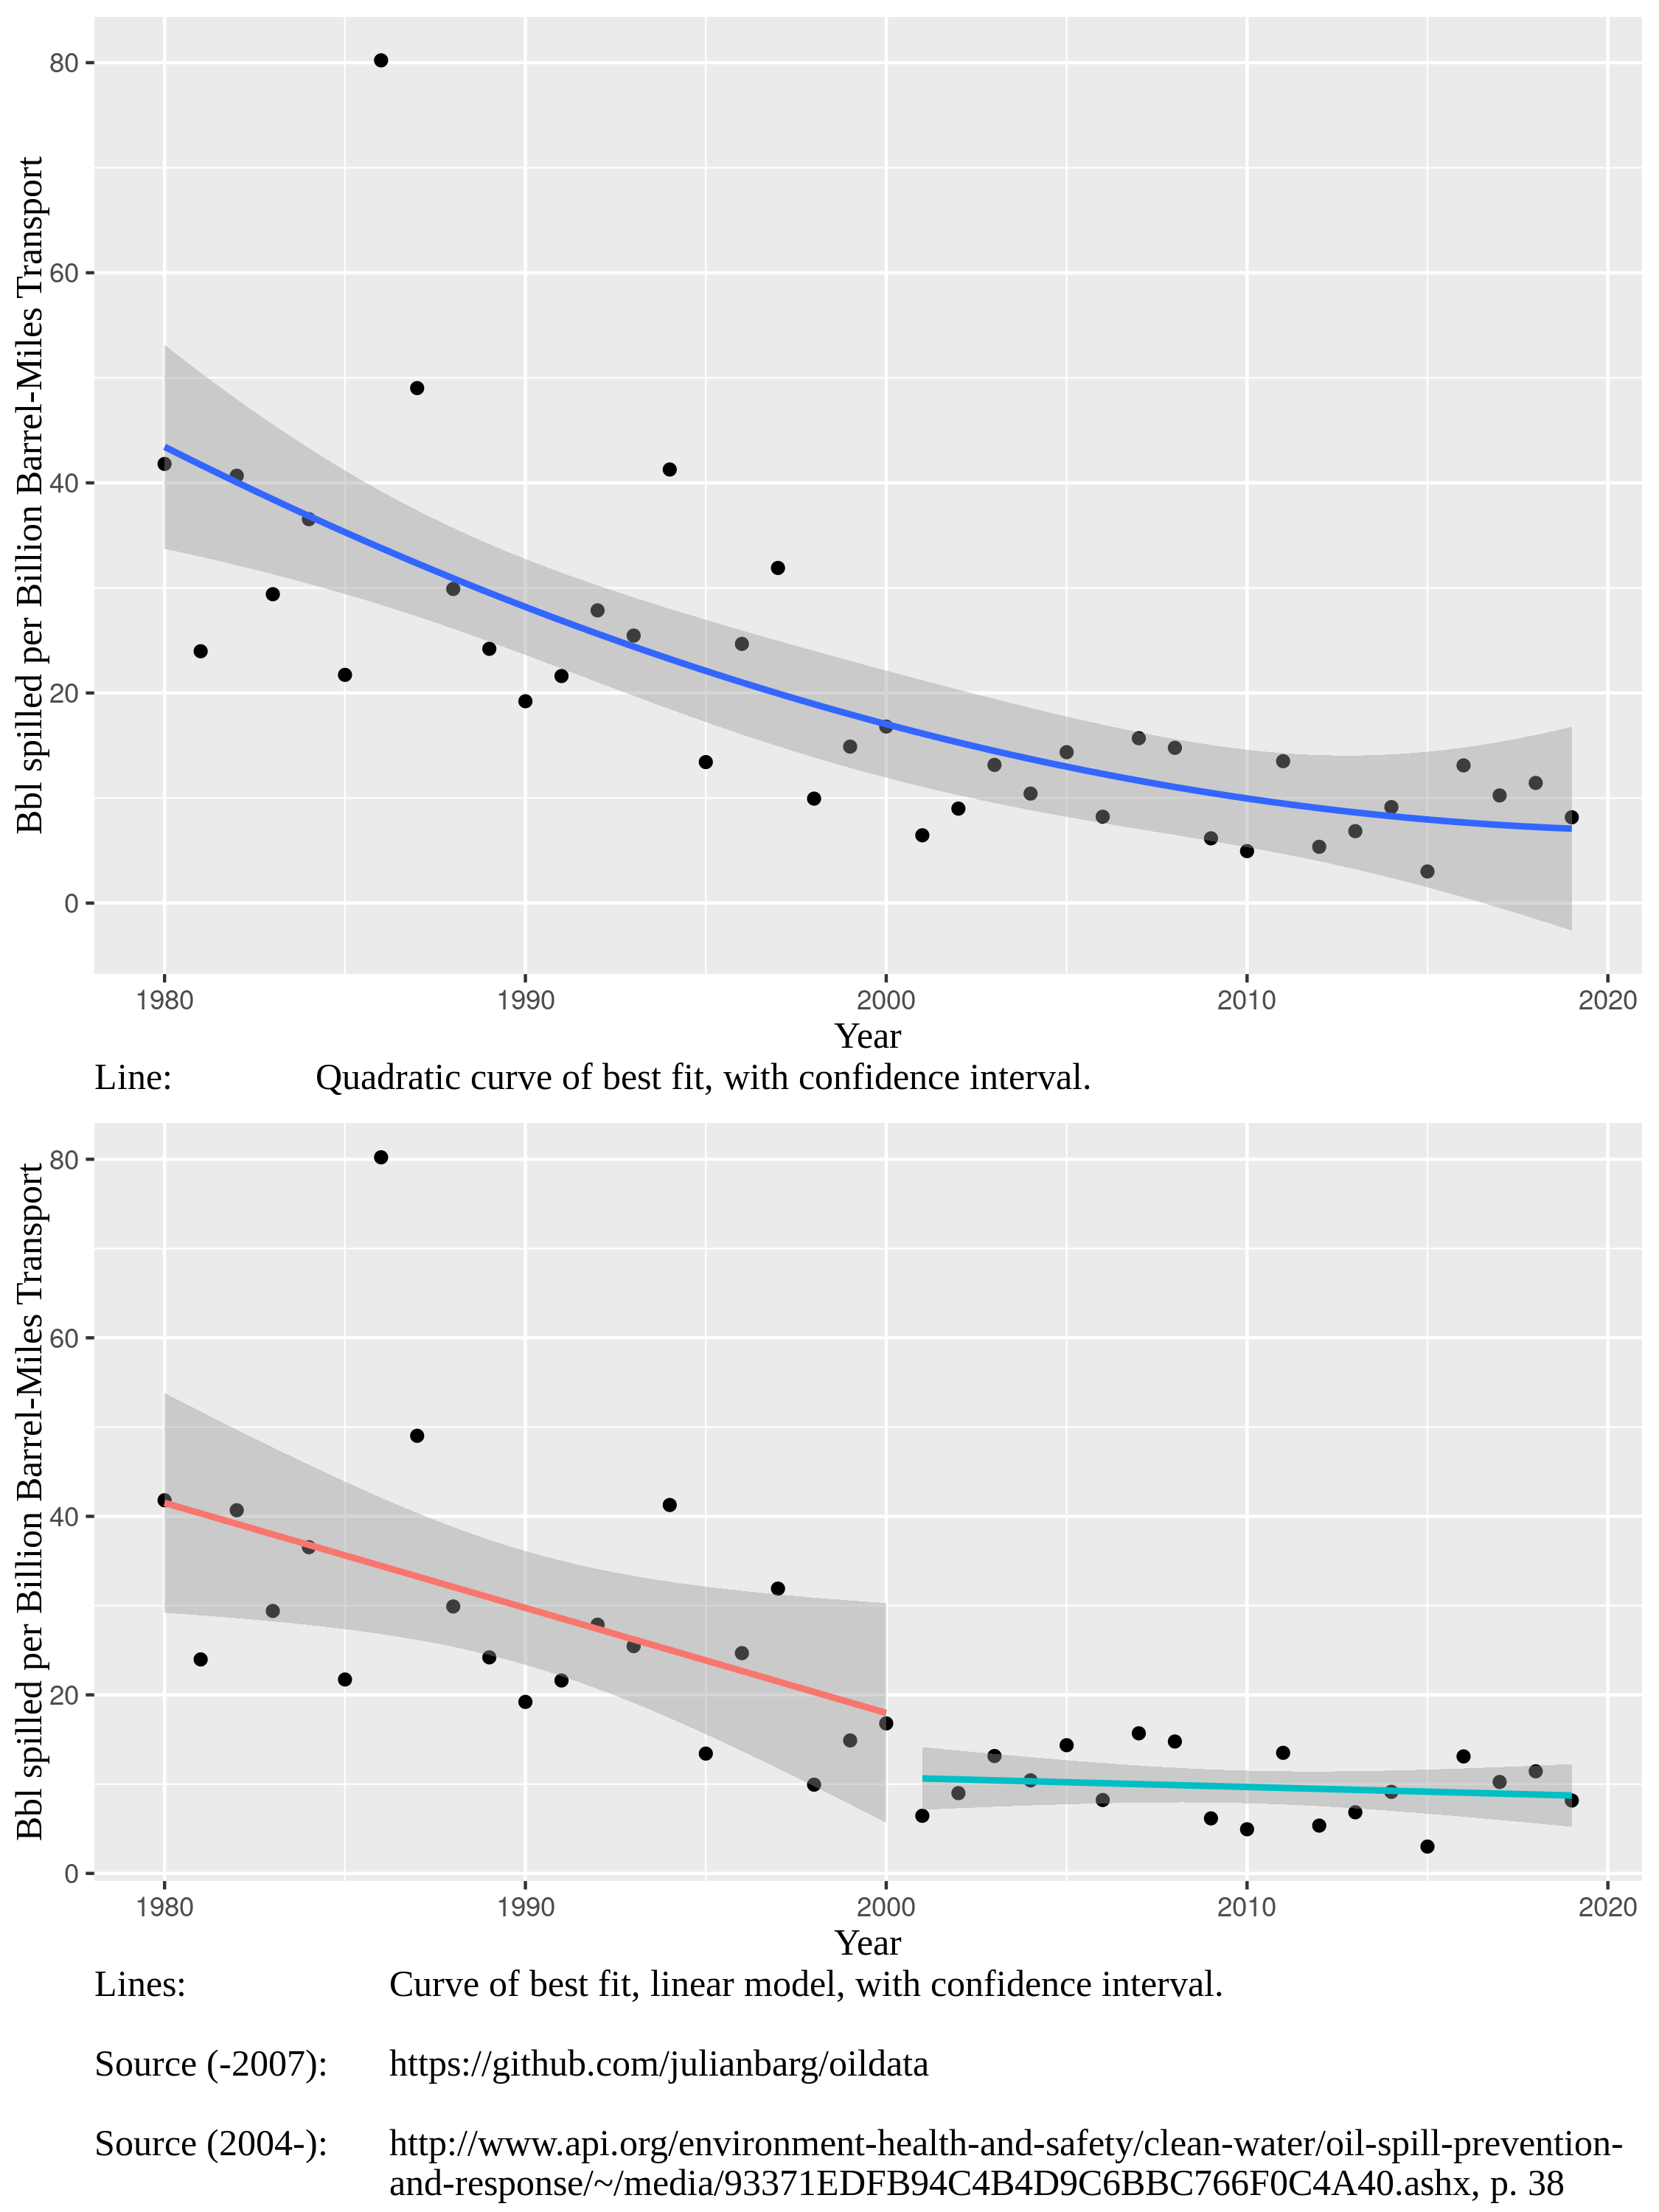
\includegraphics[scale=0.30]{population_learning_6.png}
	\note{
		We can see three things clearly. 
		
		\begin{enumerate}
			\item Crude pipelines show almost continuously improvements.
			\item Refined shows improvements into the early 2000s, then stays constant.
			\item For refined, it is hard to say whether there is one curve going on, or whether there is a decline, and then a standstill.
		\end{enumerate}
		
		Meaning that the reason for improvements in pipeline safety after 2000 is something that is specific to crude oil. Also, refined learning curve for post-2000 is indistinguishable from standstill. What has changed since the year 2000?
	}
\end{frame}

\begin{frame}
	\frametitle{Phenomenon}
	\framesubtitle{Challenge 2: To what extend to introduce the context/qualitative data}
	\textbf{Example from AOPL media campaign}
	\begin{figure}
		\centerline{
			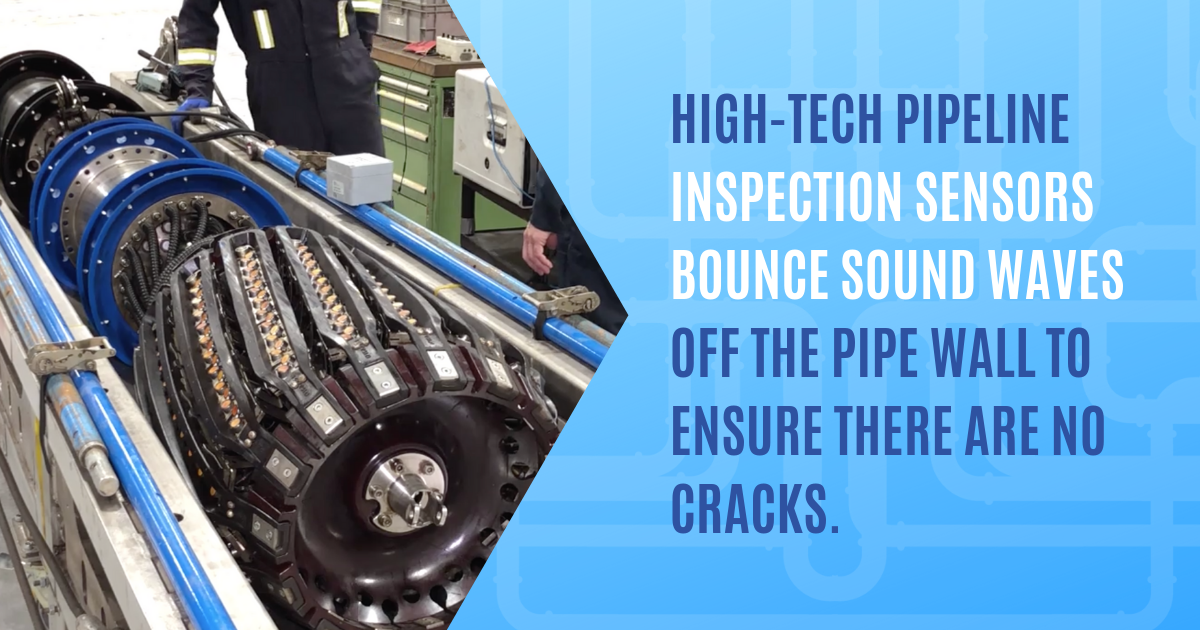
\includegraphics[scale=0.25]{tech2.png}}
		\caption{\url{https://aopl.org/305561/Page/Show?Slug=toolkit-technology}}
	\end{figure}	
	Video: \url{https://vimeo.com/366506379}
	
	\note{
		\tiny{		
		Give me your cynical response to that video. Mark, based on your experience with technology, something like TQM. My response was--this is probably the control room for training. How many operators really have these fancy new devices in mint conditions? How much more likely is it that there are devices that have not been upgraded for 20 years? Interestingly enough, even in this short excerpt we can see one of the things that the regulator would complain about. Who can really look at six screens at the same time? How many lines is this employee operating at the same time?
		
		This is where reliability comes into play. The industry very consistently communicates a set of technologies. We technology is comprehensible and approaches to problems are sensible. However, that the technology exists does not mean that it is used, or properly used. Reports such as NTSB on Kalamazoo show that there are many potential loopholes and error sources. The deeper I go into the qualitative data, the more I can show that. Guess why crude has improved and refined has not? Because coatings, that's my hypothesis why. Not the fancy technology, that is not necessarily broadly applied. Who knows how many operators really have these new decides?
		
		My best guess for the last slide as to why there are big changes for crude pipelines but not refined? Coatings! If the other technology is so great, it should also benefit refined pipelines.
		}
	}	
\end{frame}